\section{Inteligencia Artificial en Videojuegos}
\subsection{Historia}
Desde los principios de la inteligencia artificial, los expertos han dedicado una importante cantidad de tiempo y esfuerzo para construir sistemas inteligentes con el propósito de que pudiesen jugar a juegos con un nivel igual o superior al humano. Este enfoque en el estudio de los juegos se debe a que ofrecen un campo de estudio ideal para la inteligencia artificial: los juegos son problemas complejos que ofrecen desafíos para múltiples campos de la inteligencia artificial y además son tan populares que se dispone de cantidades inmensas de información sobre ellos\cite{ai_and_games}.

Los primeros programas capaces de jugar contra humanos surgieron en los años cincuenta. Uno de los ejemplos más antiguos es el algoritmo ajedrecista de Alan Turing de 1948\cite{turing_chess}, el cual era ``ejecutado'' en papel por un humano que seguía manualmente los pasos del algoritmo. El primer Software capaz de jugar a un jugo fue la inteligencia artificial para el juego \citegame{oxo}. En 1959, Arthur L. Samuel\cite{machine_learning} programo una inteligencia artificial para jugar a las Damas la cual contaba con un sistema de aprendizaje. 

Sin embargo, estos programas eran muy simples y no planteaban reto alguno contra jugadores experimentados cuando se trataba de juegos con una cierta complejidad, como el ajedrez. Hubo que esperar a los años noventa para que empezaran a surgir programas capaces de derrotar a grandes maestros de distintos juegos: en el año 1994 el programa Chinook Checkers derrotó al campeón mundial de la Damas Marion Tinsley\footnote{https://webdocs.cs.ualberta.ca/~chinook/project/} y 3 años más tarde el super-ordenador Deep Blue venció a Gary Kasparov\footnote{http://www-03.ibm.com/ibm/history/ibm100/us/en/icons/deepblue/}. Hoy en día, la inteligencia artificial ha demostrado ser capaz de superar a los jugadores humanos en casi cualquier juego, con ejemplos tales como la inteligencia artificial Watson ganando el concurso de televisión Jeopardy en 2011\footnote{https://www.youtube.com/watch?v=WFR3lOm\_xhE} o el programa AlphaGo derrotando a Ke Jie, el jugador número uno de Go\footnote{https://www.theverge.com/2017/5/25/15689462/alphago-ke-jie-game-2-result-google-deepmind-china} (un juego con una complejidad varios ordenes de magnitud superior al ajedrez).

\begin{figure}[h]
	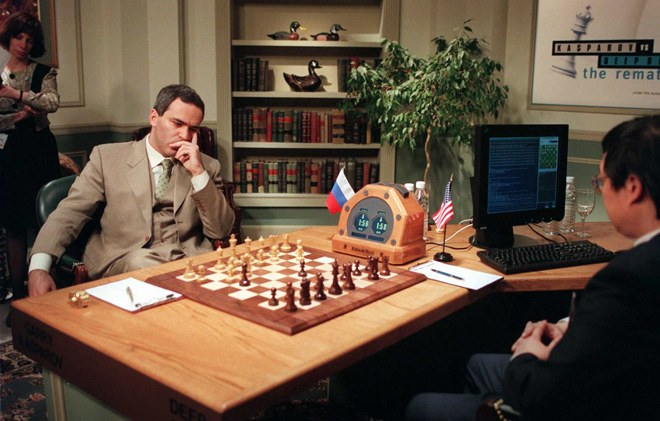
\includegraphics[width=0.8\textwidth]{images/estadodelarte/ai/deepblue-vs-kasparov}
	\centering
	\caption{El Gran Maestro de ajedrez Garri Kaspárov (izquierda) enfrentándose al ordenador Deep Blue}
\end{figure}

Hoy en día, con el auge de los videojuegos, ha comenzado el estudio para la resolución de juegos continuos en tiempo real (en contraste a los juegos de mesa tradicionales, que son discretos). Estos juegos presentan un desafió mayor, pero ya se han realizado avances, como el algoritmo desarrollado por Google DeepMind en 2014 para la resolución de varios juegos de la consola clásica Atari 2600\footnote{https://deepmind.com/research/publications/playing-atari-deep-reinforcement-learning/}.

\subsection{IA Aplicada a Videojuegos: Contexto Actual}
El uso de la Inteligencia Artificial en la industria del videojuego difiere en varios puntos a su aplicación habitual en el campo académico de los juegos que hemos visto en el apartado anterior. La principal diferencia es el tipo de problema que se intenta resolver utilizando inteligencia artificial en cada una de las ramas: en la Inteligencia Artificial aplicada a jugar a juegos se busca obtener un sistema capaz de jugar de manera óptima para derrotar a cualquier adversario humano, sin embargo, en la Inteligencia Artificial orientada a videojuegos lo que se busca es crear sistemas con los que mejorar la experiencia de juego del jugador. Esta diferencia de objetivos hace que la Inteligencia Artificial no se aplique únicamente a la creación de oponentes virtuales, sino también al modelado del comportamiento de Personajes No Jugadores y a la Generación Procedimental de Contenido\cite{ai_and_games}.

En el ámbito de los videojuegos, a la Inteligencia Artificial que interacciona con el juego como un jugador más suele llamarse "Bot". Estos bots predominan en juegos competitivos donde es necesario un oponente con un grado de inteligencia elevado para suponer un reto al jugador, como los juegos de estrategia, los juegos de lucha o los juegos de disparos en primera persona. Debido al elevado coste y complejidad de desarrollar una Inteligencia Artificial potente para estos juegos, por no hablar de la potencia requerida para ejecutarla, en la mayor parte de los videojuegos la Inteligencia Artificial ``hace trampas'', juega teniendo acceso una serie de ventajas que los jugadores humanos no tiene. Estos sistemas podrían, por ejemplo, acceder a información oculta del jugador (como la posición o recursos) a la hora de planificar estrategias o dispondrían de más y mejores recursos que sus adversarios. 

En la mayoría de los juegos, la Inteligencia Artificial no se dedica al modelado de bots como los descritos anteriormente, sino que lo más común es que se utilice para controlar el comportamiento de Personajes no Jugadores, o NPCs (siglas inglesas de Non-Player Character). Estos pueden tener comportamientos muy variados dependiendo de su papel en el juego: pueden actuar como adversarios, servir de ayuda para el jugador, formar parte de un puzle, contar una historia o simplemente formar parte del trasfondo de la acción. En el diseño de NPCs, lo que se busca son dos cosas: crear una Ilusión de Inteligencia, de forma que los jugadores crean que el NPC es un ser inteligente, aunque sea controlado por un código muy sencillo, y, en especial con adversarios, que sea predecible, de forma que el jugador pueda desarrollar estrategias para enfrentarse/interaccionar con ellos.

\begin{figure}[h]
	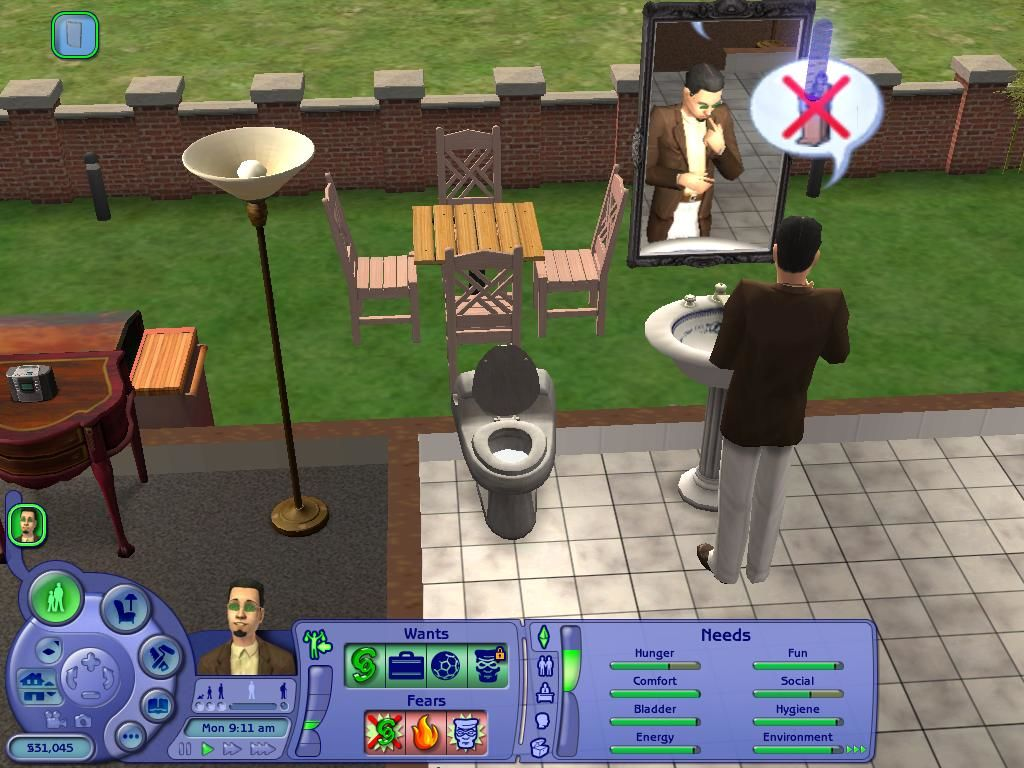
\includegraphics[width=0.8\textwidth]{images/estadodelarte/ai/sims-captura}
	\centering
	\caption{En \citegame{sims}, los personajes pueden tomar decisiones basándose en sus gustos y necesidades.}
\end{figure}

La otra aplicación principal en los videojuegos es la Generación Procedimental de Contenido. La generación Procedimental de Contenido es el nombre que reciben los métodos que permiten generar el contenido de un juego de forma automática o con solo un mínimo de intervención humana. Actualmente, la mayor parte de los juegos que hacen uso de la generación procedimental la utilizan para la creación automática de mapas o niveles o para la creación de objetos. La generación procedimental de contenido puede utilizarse tanto como una herramienta durante el desarrollo, que serviría para generar contenido que luego sería refinado por los desarrolladores; o podría formar parte del juego final, generando nuevo contenido al gusto del jugador de forma automática.

\begin{figure}[h]
	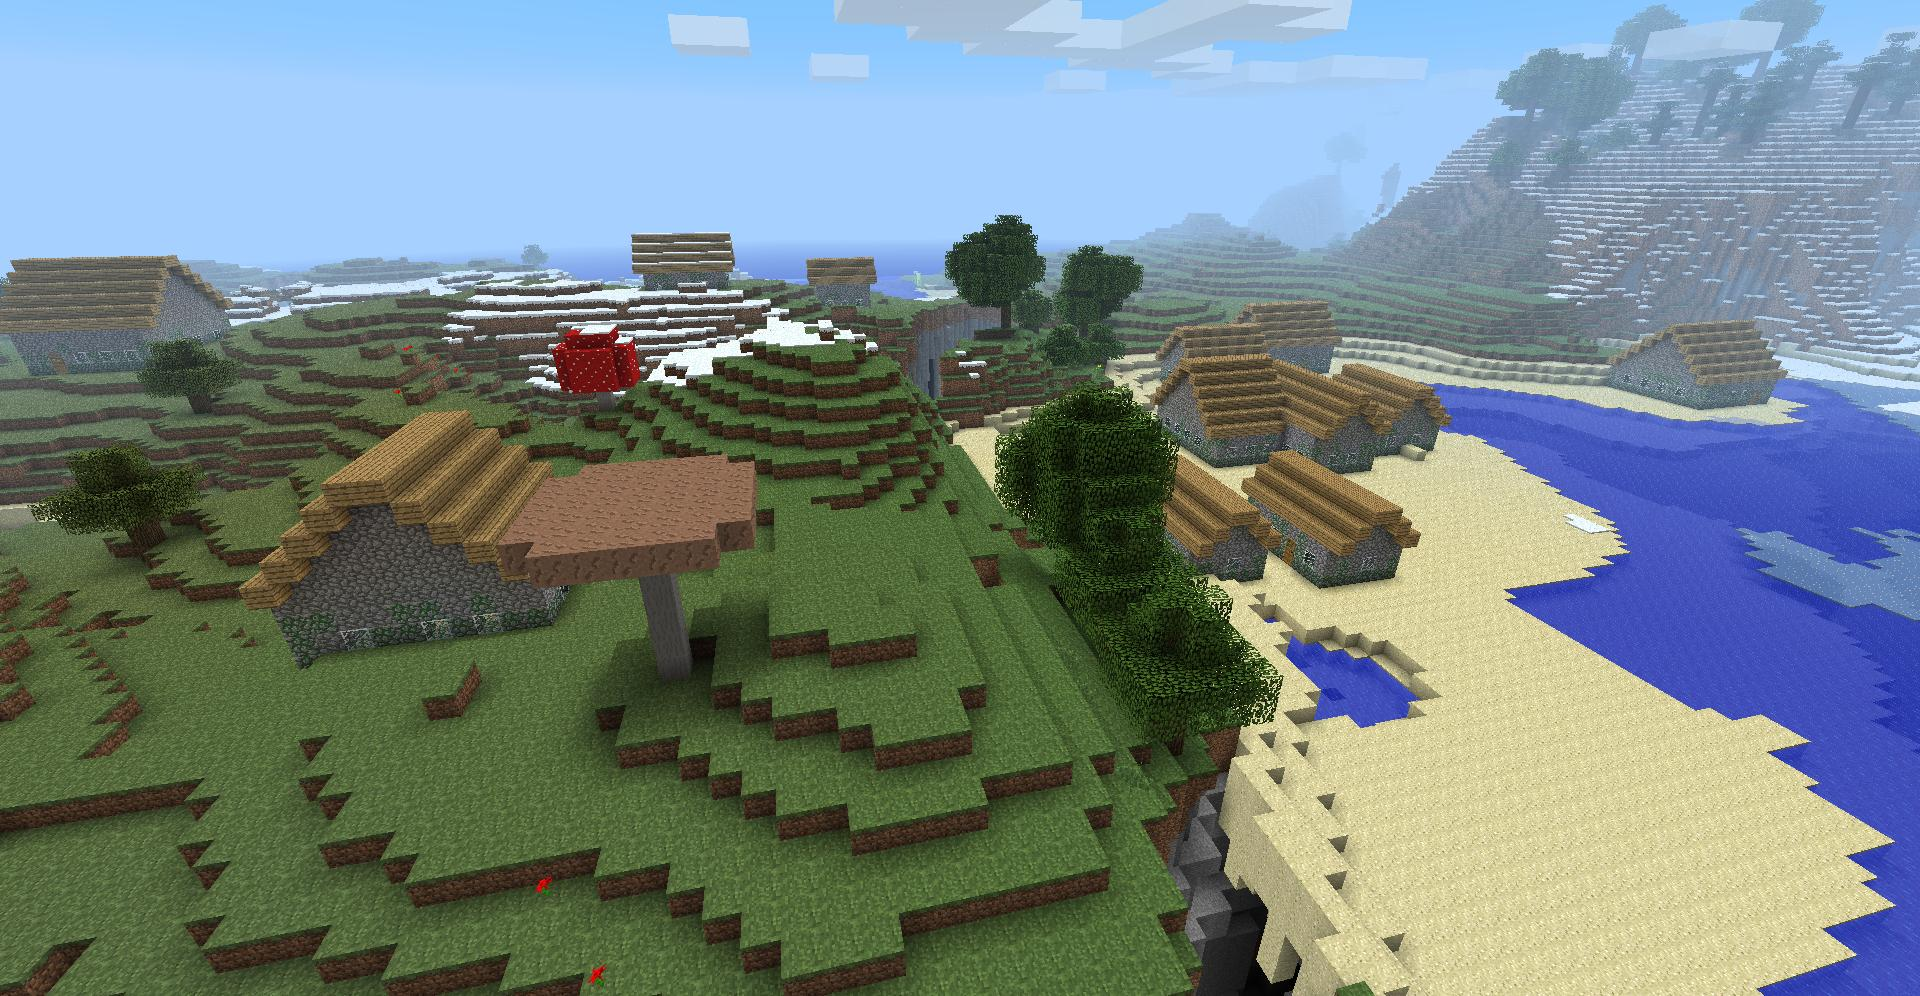
\includegraphics[width=0.75\textwidth]{images/estadodelarte/ai/minecraft}
	\centering
	\caption{\citegame{minecraft} es un ejemplo claro de generación procedimental de terrenos.}
\end{figure}

\subsection{Métodos de la IA}
Existen varios tipos de métodos y algoritmos los cuales pueden ser utilizados para construir inteligencias Artificiales. La elección entre los distintos tipos de métodos debe realizarse dependiendo del tipo de problema que se intenta resolver y de los recursos de los que se dispone, tanto las prestaciones del dispositivo en el que van a ser implementados como margen de tiempo máximo de la ejecución del algoritmo\cite{ai_and_games}. 

Los Métodos de la inteligencia artificial pueden ser agrupados en las siguientes categorías, debido a sus características y aplicaciones similares:

\subsubsection{Métodos Ad Hoc}
Esta clase de métodos de IA es una de la primera y, en el sector del videojuego, la más común. Su nombre proviene de la locución latina que, traducida, significa ``para esto'', y hace referencia a que se tratan de soluciones precisas para problemas concretos, las cuales no pueden generalizarse ni aplicarse a otros problemas distintos\cite{ai_and_games}.

Pese al notable problema que provoca la falta de reusabilidad de estos métodos, son los más utilizados en el desarrollo de videojuegos. Esto se debe a que, por lo general, son muy fáciles de diseñar, visualizar, implementar y depurar; además requerir de muy pocos recursos cuando se aplican a problemas pequeños.

Algunos tipos de métodos Ad hoc son:
\begin{itemize}
\item \textbf{Máquinas de estados finitos}: Es un tipo de sistema experto en el que la información es representada por un grafo dirigido, donde los nodos representan \textbf{Estados} en los que se puede encontrar un comportamiento, proceso o algoritmo y las aristas  las \textbf{Transicciónes} condicionales entre los distintos estados. Fácil de diseñar e implementar, pero su complejidad crece muy rápido, por lo que no es apto para problemas grandes.
\item \textbf{Arboles de comportamiento}: Este tipo de sistema experto utiliza una estructura en árbol para el modelado de información, donde cada nodo es un \textbf{comportamiento}. El algoritmo recorre el árbol en profundidad, ejecutando el comportamiento de dicho nodo. El comportamiento del nodo padre depende del resultado de los hijos. Los arboles de comportamiento ofrecen una mayor flexibilidad que las máquinas de estados a cambio de mayor complejidad.
\item \textbf{IA basada en utilidad}: Esta técnica se basa en el uso de una \textbf{Función de Utilidad}, la cual asigna un valor de utilidad a todas las opciones del agente inteligente basándose en información del entorno. El agente elije la opción que tenga una utilidad más alta.
\end{itemize} 

\subsubsection{Búsquedas en Árbol}
Una de las bases de la inteligencia artificial son los \textbf{algoritmos de búsqueda en árbol} son una de las bases de la inteligencia artificial, dado que la mayor parte de los problemas de la inteligencia artificial podrían plantearse usando este tipo de algoritmos\cite{ai_and_games}.

La búsqueda en árbol consiste en la construcción de un \textbf{Árbol de búsqueda}, un tipo de grafo dirigido en el cual los nodos o hojas representan estados mientras que las aristas o ramas representan las acciones que provocan la transición de un estado a otro. El agente inteligente recorre el árbol partiendo del nodo raíz buscando la secuencia de ramas que resuelvan el problema siguiendo un algoritmo concreto. Cuando se aplican a juegos, los arboles de búsqueda suelen aplicarse para modelar el estado del juego: la inteligencia artificial recorre el árbol buscando la secuencia de acciones que lleve al estado de victoria, o evitando el estado de derrota.

Existen numerosos algoritmos de búsqueda distintos, los cuales pueden agruparse en las siguientes categorías:
\begin{itemize}
\item \textbf{Búsqueda no informada}: Se trata de los algoritmos más básicos, en los que se realiza la búsqueda sin ningún tipo de información adicional sobre el objetivo. Sus variantes más simples son el algoritmo \textbf{Primero en Anchura}(explora todas las acciones de un estado antes de pasar al siguiente) y el \textbf{Primero en Profundidad}(explora una secuencia de ramas todo lo que puede antes de volver e intentar otra secuencia distinta)
\item \textbf{Búsqueda Primero el Mejor}: En estos algoritmos se cuenta con información adicional sobre el nodo objetivo, la cual se utiliza para determinar que nodos deben explorarse primero. Un tipo de algoritmos Primero el Mejor son los algoritmos \textbf{A*}, en los cuales los nodos se seleccionan basándose en su \textbf{Coste}(suma de la distancia entre el nodo y el nodo raíz y la distancia estimada al objetivo.
\item \textbf{Búsqueda MiniMax}: Este tipo de algoritmos se utilizan para resolver problemas que involucran a dos adversarios enfrentados. En estos algoritmos se va alternando entre jugadores \textbf{Min y Max}, los cuales intentan llegar a sus respectivos estados de victoria opuestos. El espacio de búsqueda de estos algoritmos suele ser muy grande, por lo que suelen usar funciones de evaluación para evitar recorrer el árbol de búsqueda completo.
\item \textbf{Árbol de búsqueda de Monte Carlo}: Se trata de una familia de algoritmos diseñados para resolver problemas \textbf{No deterministas} y/o de \textbf{Información Imperfecta}. Para evaluar la calidad de un estado dado, el algoritmo utiliza simulaciones aleatorias de partidas a partir de ese estado. La siguiente acción será con la que empezó el mayor número de partidas victoriosas.
\end{itemize} 

\subsubsection{Algoritmos de Optimización}
Los algoritmos de optimización, a diferencia de la búsqueda en árbol, se centran en obtener una solución correcta, ignorando los pasos que llevaron a esta. Para ello, el algoritmo empieza tomando una solución sub-optima, la cual va modificando en múltiples iteraciones utilizando una \textbf{función de Aptitud} como guía hasta obtener una solución con una Aptitud máxima\cite{ai_and_games}.

Existen varios tipos de algoritmos de optimización, dependiendo de los métodos que elijan para la selección de la solución inicial, para la evaluación de aptitud o para la modificación:
\begin{itemize}
\item \textbf{Búsqueda Local}: Este tipo de algoritmos consisten en, dada una solución, revisar todas las soluciones que difieran de dichas soluciones por una distancia mínima. Si alguna de las soluciones mejora a la solución original, se remplaza la solución original por la nueva solución y repite el algoritmo; si no, la solución original es elegida como la solución óptima.
\item \textbf{Algoritmos Evolutivos}: Los algoritmos Evolutivos son un tipo de algoritmos de optimización basados en la evolución por selección natural Darwiniana que se observa en la naturaleza. Su funcionamiento se basa en un conjunto amplio de soluciones candidatas. EN cada iteración del algoritmo, las distintas soluciones se ``cruzan'' para obtener soluciones mixtas, las cuales son evaluadas. Finalmente, se forma un nuevo conjunto de soluciones a partir de las soluciones más exitosas. El algoritmo se repite hasta obtener la solución más óptima.
\end{itemize} 

\subsubsection{Aprendizaje Automático}
El aprendizaje automático es una rama de la computación que permite dotar a los ordenadores de la capacidad de ``aprender'' a realizar una tarea utilizando datos en lugar de programarlo específicamente para esa tarea\cite{machine_learning}. Los algoritmos de aprendizaje automático suelen aplicarse a problemas donde es muy difícil, o incluso imposible, programar un algoritmo implícito que pueda resolverlo, como por ejemplo el filtrado de correos o la visión por ordenador.

Una forma de clasificar los algoritmos de aprendizaje automático es basándose en el tipo de \textbf{Retroalimentación} que reciben. De esta forma, surgen las siguientes categorías:
\begin{itemize}
\item \textbf{Aprendizaje Supervisado}: Se trata de algoritmos que extraer los atributos y características comunes de los integrantes de grupos etiquetados. Estos algoritmos funcionan recibiendo conjuntos de muestra formado por datos etiquetados en distintos grupos y categorías. Analizando los conjuntos de muestra, el algoritmo debe ser capaz de asignar nuevos datos a la categoría correcta. Existen muchos tipos de algoritmos de Aprendizaje supervisado, como por ejemplo las \textbf{Redes Neuronales}, que funcionan imitando la estructura de las neuronas del cerebro.
\item \textbf{Aprendizaje por Refuerzo}: Los algoritmos de Aprendizaje por Refuerzo se inspiran en el \textbf{Conductismo Psicológico}, basándose en la forma en la que los animales aprenden a tomar decisiones basándose en los estímulos positivos y negativos de su entorno. Estos algoritmos suelen implementarse mediante un agente inteligente que interacciona con un entorno mediante acciones. Con cada acción, el agente recibe un estímulo positivo o negativo, que almacena con la intención de descubrir la secuencia de acciones que maximice el estímulo positivo a largo plazo mediante técnicas similares a los algoritmos de Optimización
\item \textbf{Aprendizaje No Supervisado}: El aprendizaje No Supervisado son un conjunto de algoritmos que sirven para encontrar asociaciones y patrones en un conjunto de datos sin ningún tipo de información de refuerzo adicional. Existen varias aproximaciones a este tipo de algoritmos, como el \textbf{Clustering}, que consiste en agrupar elementos de un conjunto basándose en su similitud entre ellos y su diferencia con el resto de grupos.
\end{itemize} 

\subsection{Futuros campos de aplicación}
La Inteligencia Artificial orientada a juegos evoluciona de manera paralela a los propios videojuegos, que viven ahora más que nunca una época dorada debido al aumento constante tanto en popularidad y prestigio, lo que supone una mejora tanto en la potencia de las máquinas que los ejecutan como en las técnicas que se utilizan en su desarrollo. Esta situación cambiante ha causado la aparición de nuevos problemas que se esperan poder solucionar con el uso de técnicas de inteligencia artificial.\cite{ai_and_games} A continuación mencionaremos algunos de los futuros campos de aplicación de las técnicas de inteligencia artificial:

Una las posibles aplicaciones de la Inteligencia Artificial es la de realizar \textbf{Testing} de juegos. El programa jugaría a los juegos en busca de fallos tanto informáticos como de diseño (como problemas de balanceo o maneras de hacer trampas en el juego) de forma automatizada, ahorrado una gran cantidad de trabajo a los desarrolladores. Aunque ya existen herramientas que ofrecen una forma rudimentaria de testing automático, aun es necesario mejorar aspectos como la categorización de los errores encontrados.

La \textbf{Minería de Datos de Juego} es otro uso prometedor de la Inteligencia Artificial. Se trata de una técnica alternativa al testing habitual de juegos en la que se recolecta y analiza la información de comportamiento de la base de jugadores de un juego dado con el fin de mejorar dicho juego\cite{ai_revisited}. Esta técnica se ha popularizado gracias a la proliferación de juegos con un fuerte componente online que facilita la recogida de datos. Sin embargo los volúmenes de datos con los que se trabaja son tan masivos que los algoritmos de mineria de datos actuales no son capaces de analizarlos completamente \cite{ai_revisited}.

La \textbf{Dirección de Juegos} consiste en una Inteligencia Artificial que modifica eventos del juego en tiempo real basándose en las reacciones de los jugadores con acciones tales como modificar la dificultad, reproducir música y sonido o modificar el entorno con tal de mejorar la experiencia del jugador. Actualmente, los juegos que mejor ha implementado un sistema con esta propiedad es la saga Left 4 Death de Valve\footnote{http://www.l4d.com/blog/}. Se trata de una rama con mucho potencial que aún no ha sido explorado completamente.

Finalmente, una tarea de gran importancia para los juegos online, a pesar de no formar parte de los juegos en si, es la \textbf{motorización de los chats}. El gran volumen de mensajes que se envían a través de los chats de los juegos online más populares hace que sea imposible la moderación manual, lo que crea un entorno de juego toxico para los jugadores. Compañías como Riot Games están empezando a utilizar algoritmos de aprendizaje automático para entrenar sistemas para detectar y eliminar los mensajes inapropiados de los chats \footnote{https://www.nature.com/news/can-a-video-game-company-tame-toxic-behaviour-1.19647}.

\begin{figure}[h]
	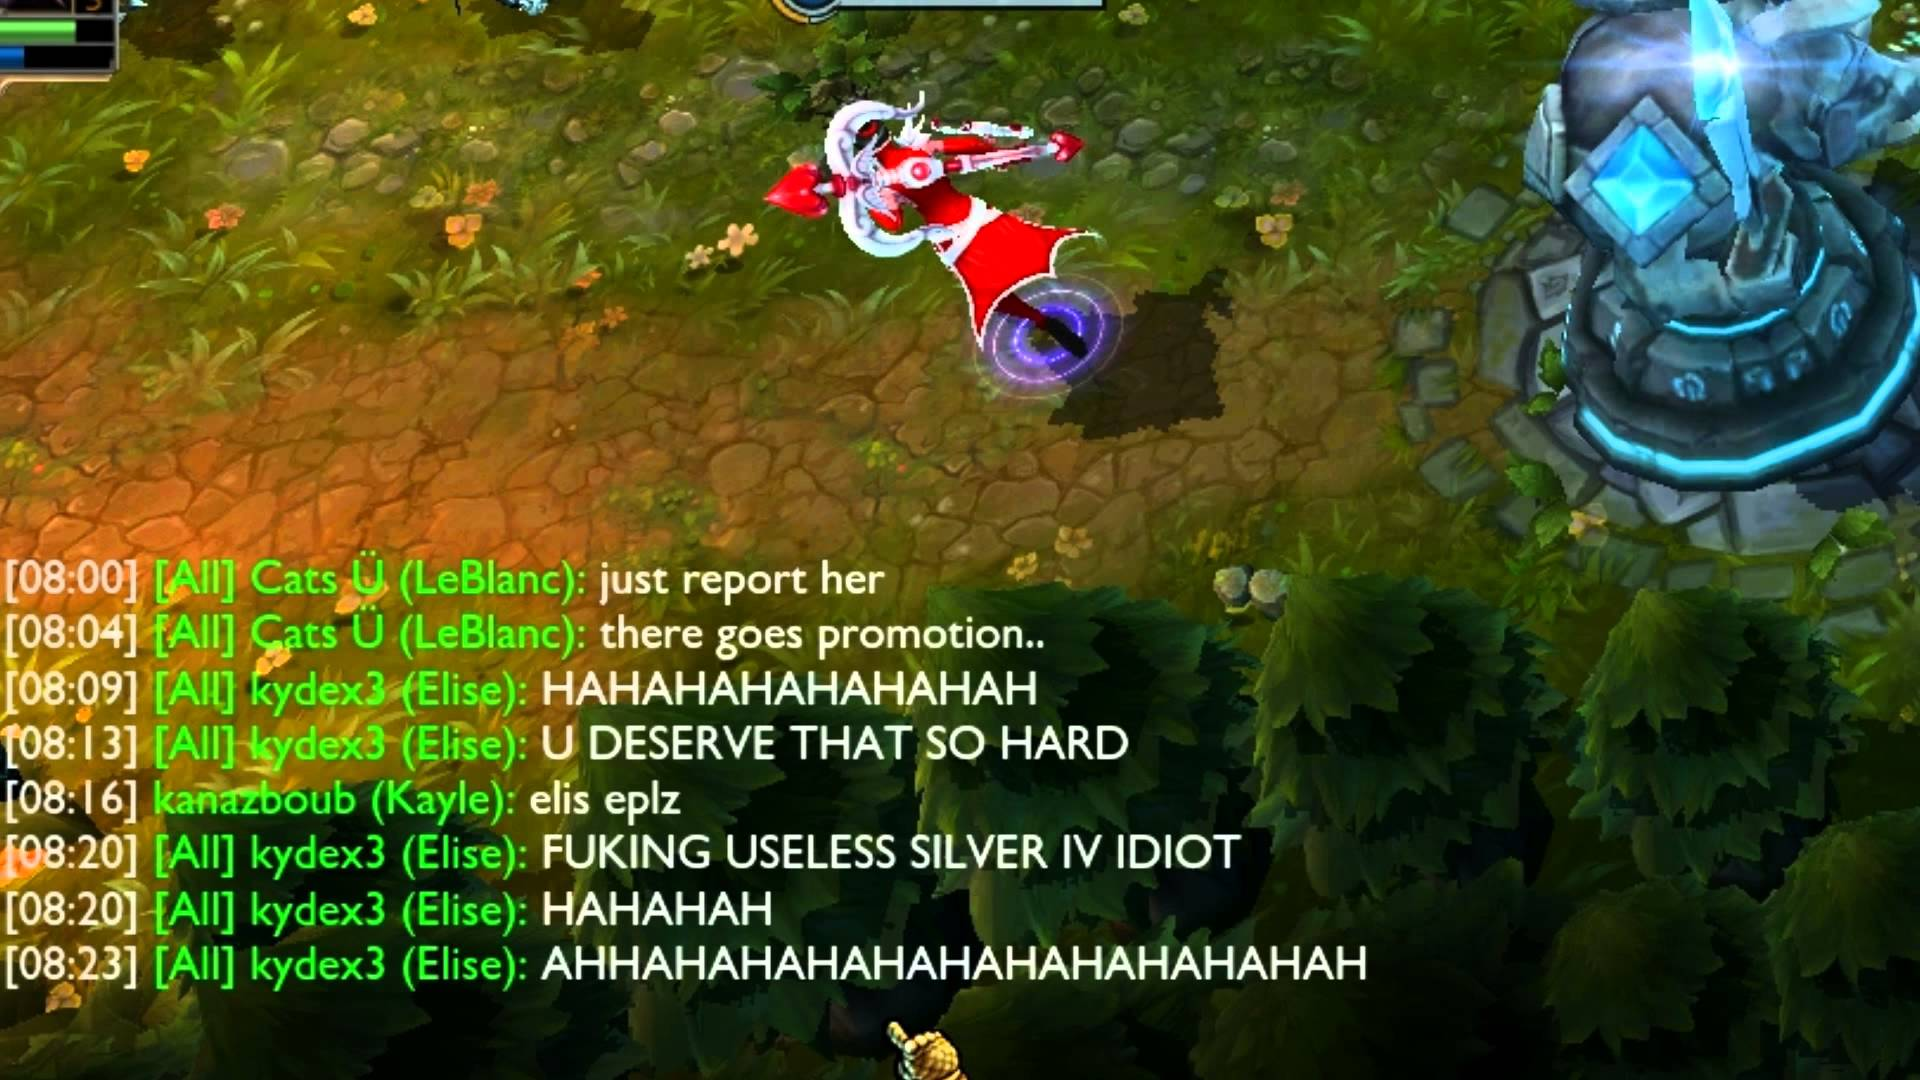
\includegraphics[width=0.45\textwidth]{images/estadodelarte/ai/lol-toxic-capture}
	\centering
	\caption{Ejemplo de comportamiento tóxico en \citegame{league_of_legends}.}
\end{figure}